\section{Symbolic \& Concolic Execution}


If we compute the symbolic constraints per path, and then solve these constraints we will have all concrete inputs that explore all paths. This is the core idea of symbolic execution.

\begin{center}
	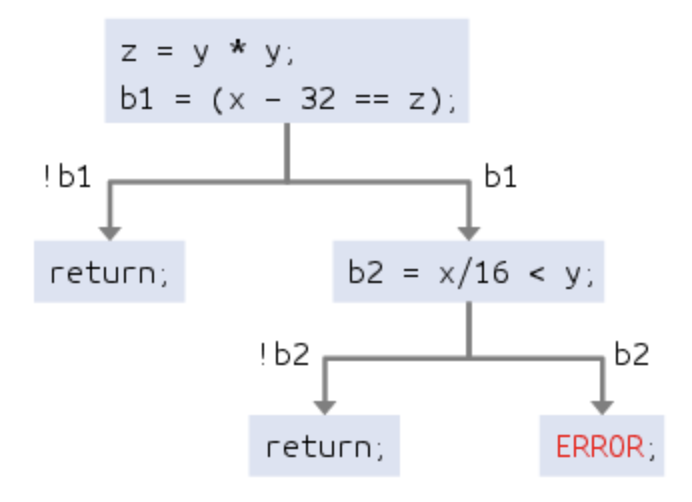
\includegraphics[width=0.5\columnwidth]{assets/path}
\end{center}

A symbolic store $\sigma$ maps variables to symbolic expressions, which are updated by assign statements. Path conditions $\pi$ are the conditions under which a path is taken. Combined we have a symbolic state per program point.
\begin{center}
	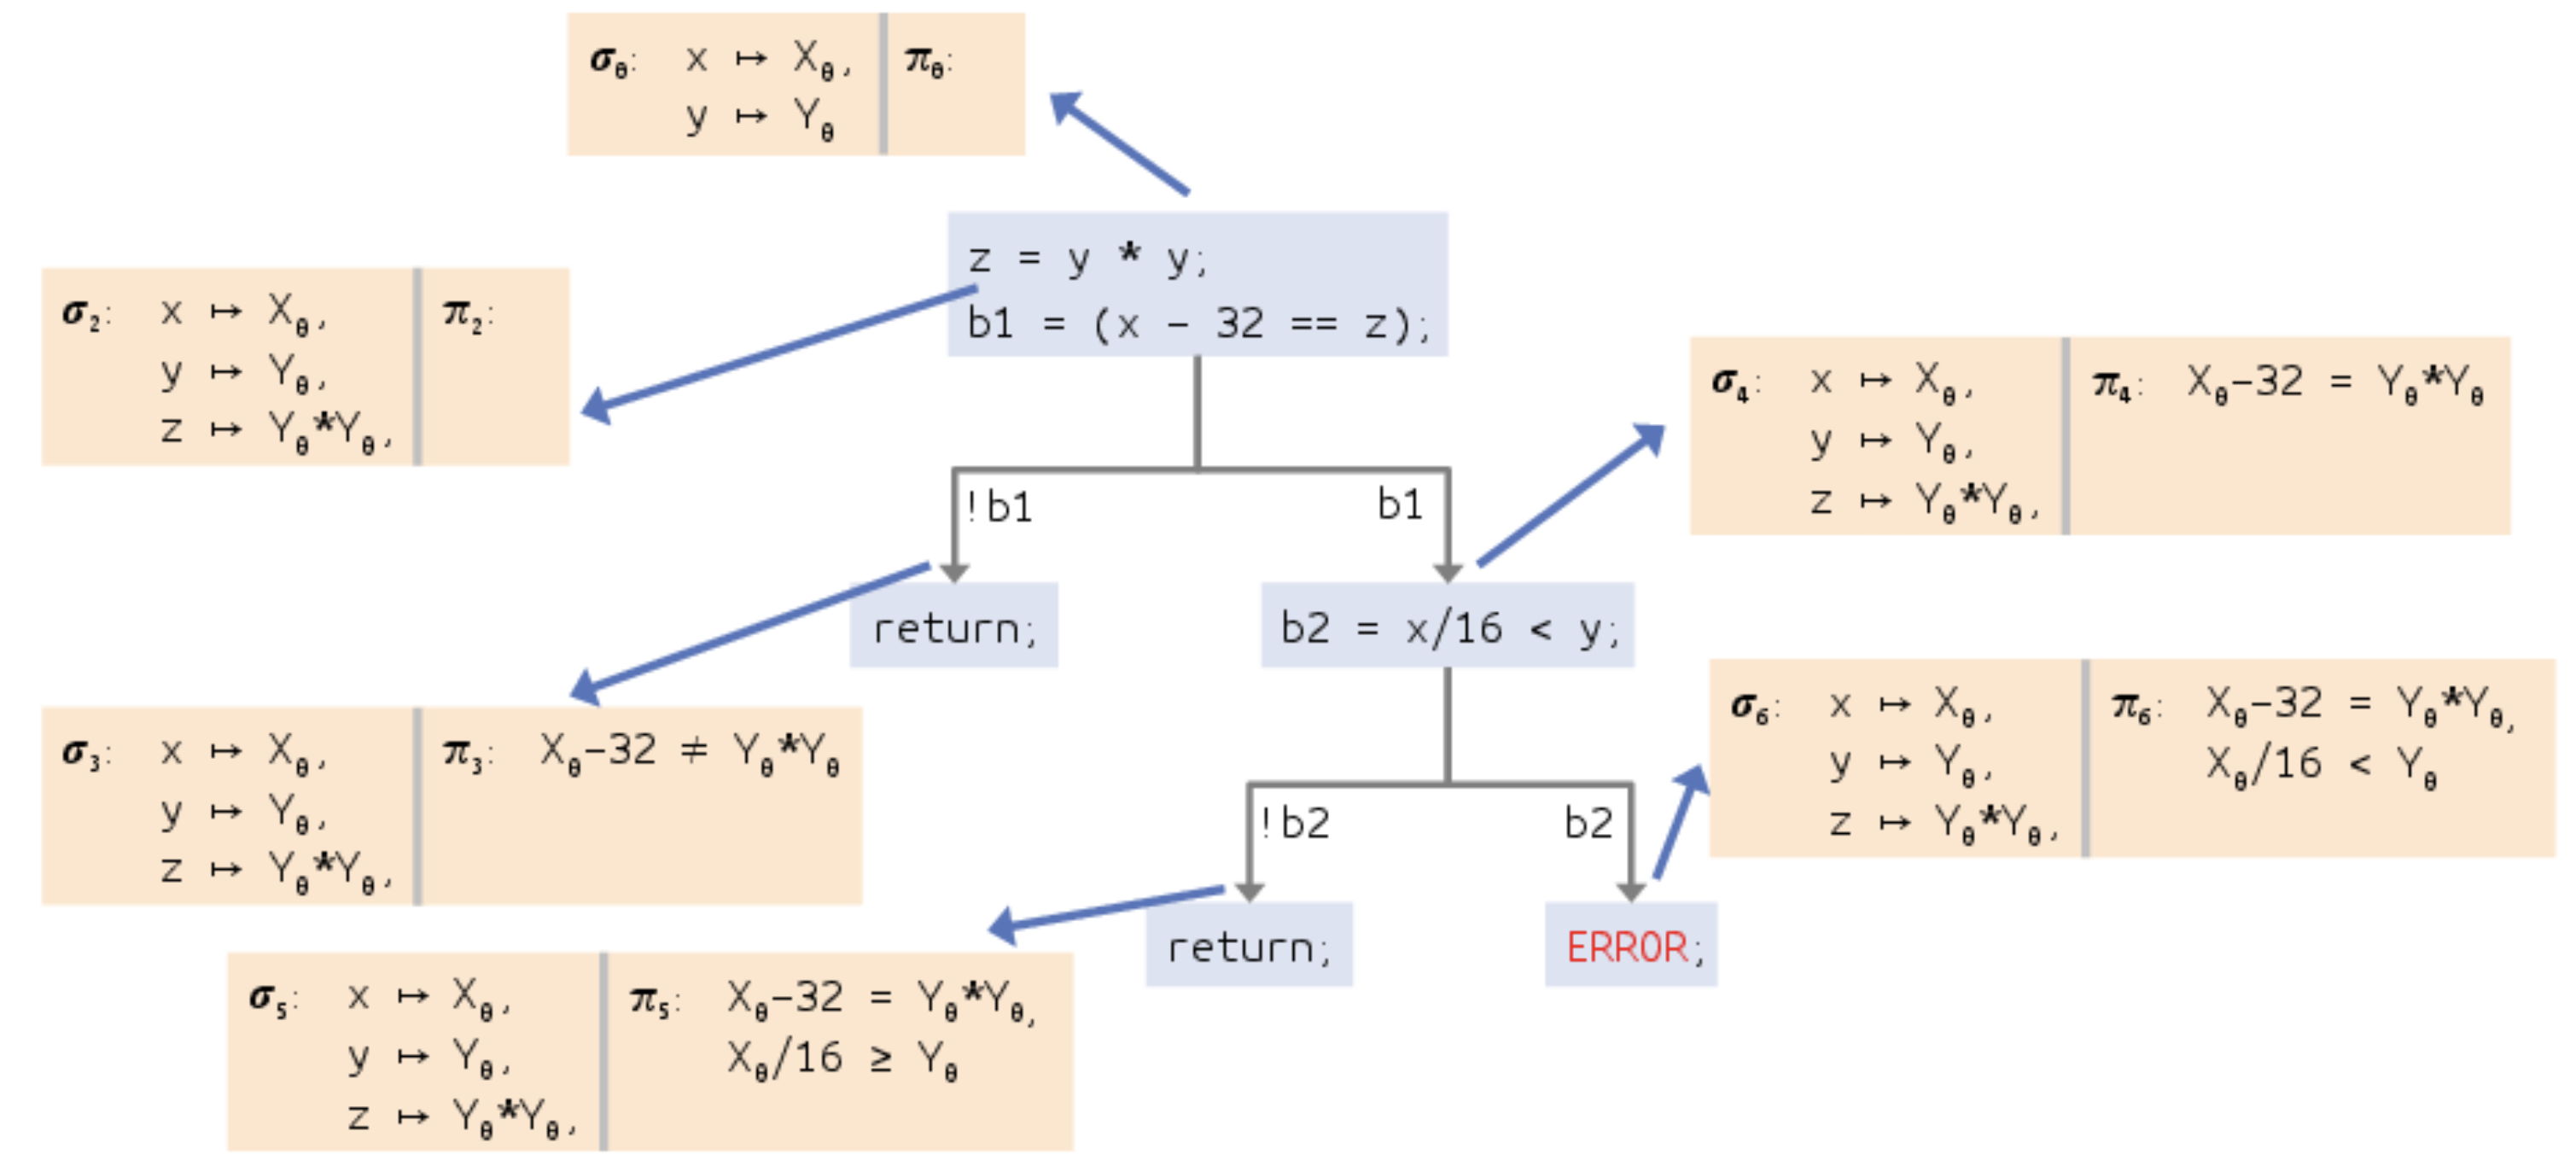
\includegraphics[width=\columnwidth]{assets/symbolic_execution}
\end{center}

Solving the final constraint sets, we can conclude which path will be taken for an input. \\

Eagerly exploring all paths up-front may include many infeasible paths and can be too time consuming. Symbolic execution engines therefore apply different exploration strategies. \\

SMT solvers combine SAT-solving with theory reasoning. They can produce models, satisfying assignments. However, there are limits. Many theories are not decidable, e.g. non-linear integers. Let us assume the solver fails to find a model for $b_1$ or $!b_1$, therefore we will not get concrete test inputs and cannot determine if the branch is infeasible. \\

Concolic execution combines concrete and symbolic execution. The high-level idea is that the concrete execution drives the symbolic one. Programs are executed with concrete inputs, but additionally maintain a symbolic state. Concrete values are used to simplify path conditions. \\

A concolic execution may not be able to explore all paths, but any additionally explored path increases the chances of uncovering bugs. We use concolic execution to expand sets of manually determined test inputs. \\

Symbolically executing native code is difficult if not impossible. Concolic execution can help by invoking the functions with concrete values. Still, it might not be able to explore all paths. \\

Further, one has to consider that symbolic expressions can become large, in particular along deep paths. Optimizations typically employed compilers are subexpression elimination and constant folding.


\subsection{Fuzzing and Symbolic Execution for Smart Contracts}

The idea behind fuzzing is to run programs on abnormal inputs (e.g. randomly generated). This should help finding potential exploits that attackers could use. \\

We want to find transactions that thoroughly explore the state space. The problem is the exponential number of block states. Both, symbolic execution and fuzzing, have their drawbacks. Imitation learning based fuzzers try to solve these problems.
\begin{center}
	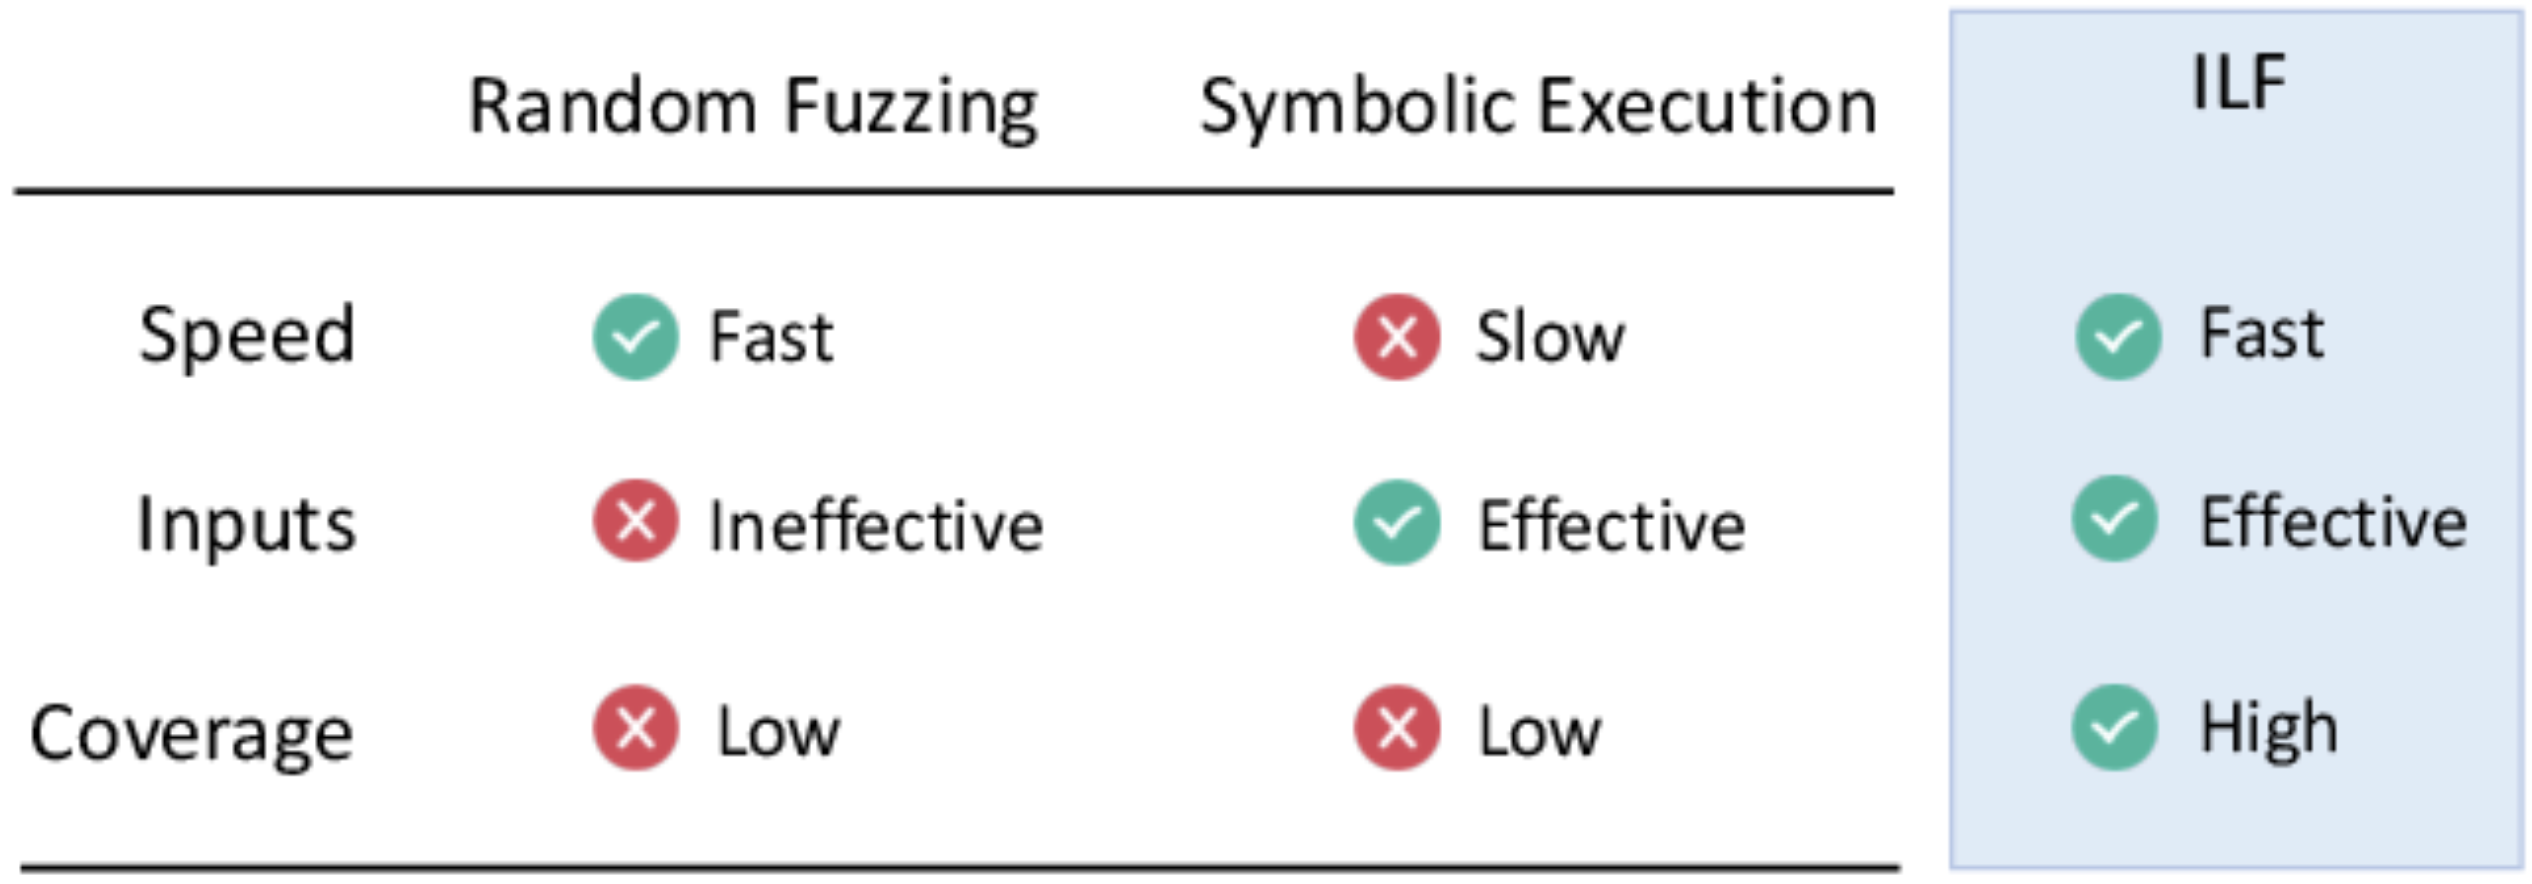
\includegraphics[width=0.9\columnwidth]{assets/fuzzing}
\end{center}

A neural network is used to learn to fuzz from symbolic execution.
\begin{center}
	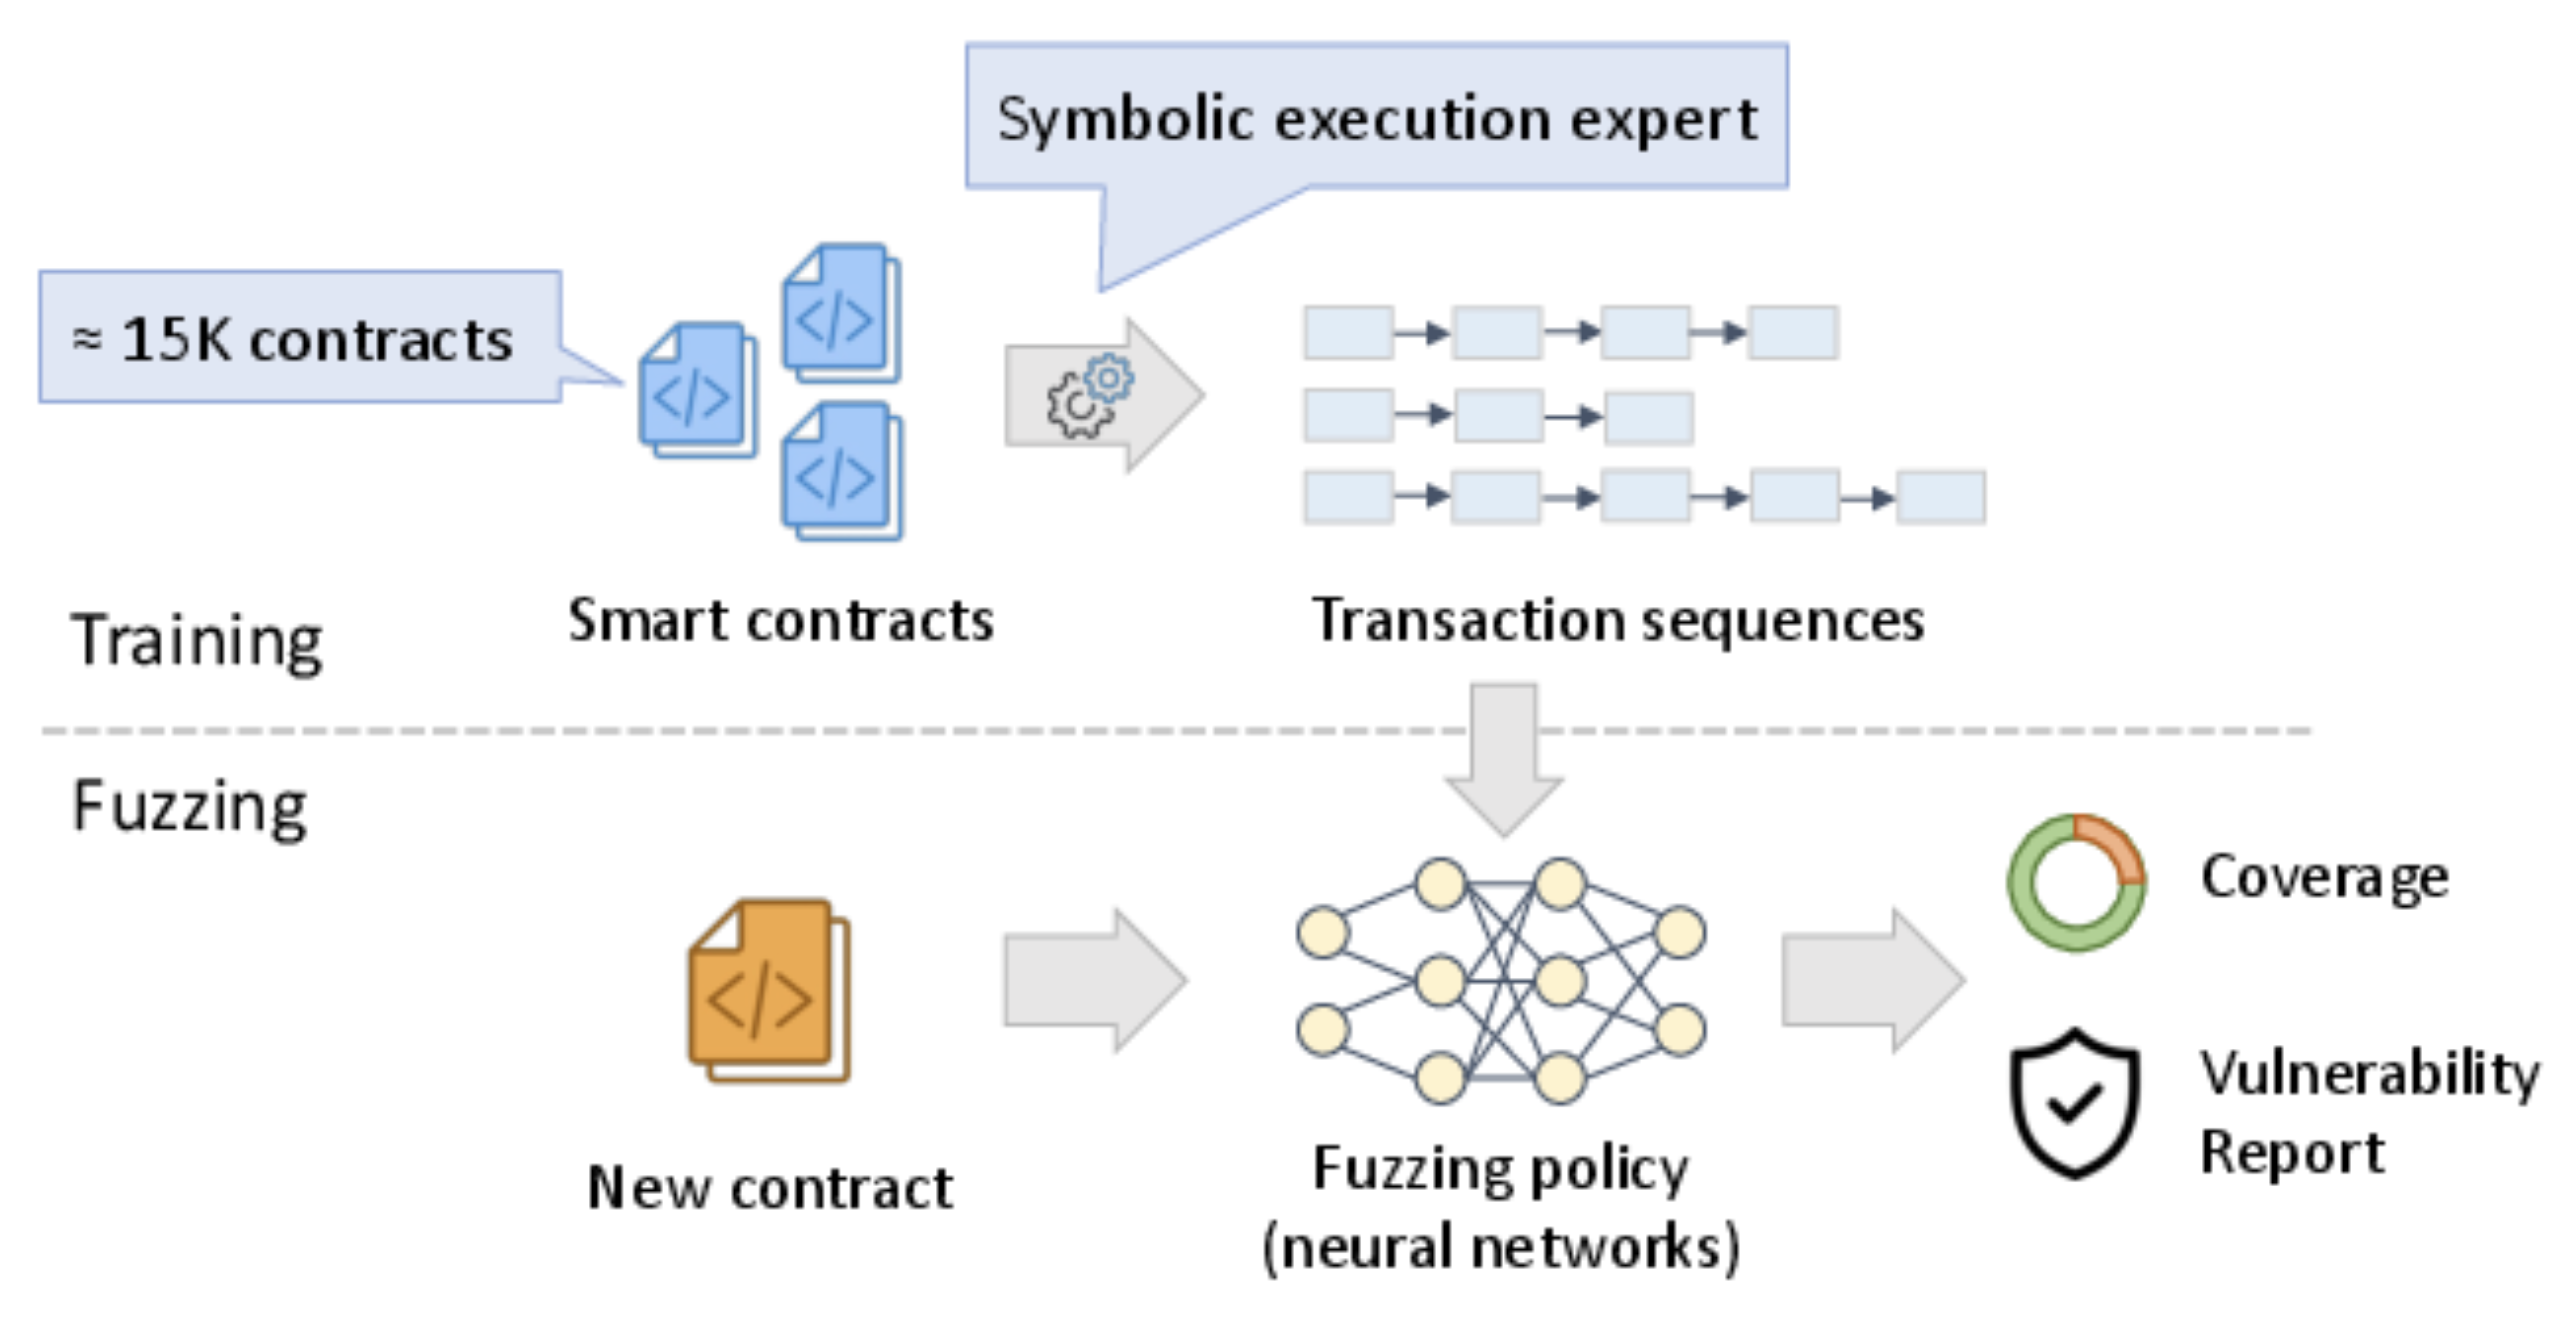
\includegraphics[width=0.9\columnwidth]{assets/ilf}
\end{center}

This approach performs better than anything comparable.